\setchapterpreamble[u]{\margintoc}
\chapter{The Transition Needs}
\labch{transition_needs}

In this chapter I will assess the situation as it is for several representative countries, each representing a different economical, geographical and energetic contexts.

\begin{description}
	\item[France] France will be taken to represent Europe as well as a large existing nuclearized electricity grid.
	\item[United States of America] The USA will be considered due to its socio-economic importance, and its varied geographical and energetic landscape.
	\item[Brazil] Brazil will also be used as a case study, a large South American country powered notably by hydroelectric power.
	\item[China] China has an immense impact on the world, and is today one of the main source of carbon emission\sidenote[][*1]{We will come back to that, but keep in mind that this is very misleading, and that it wildly depends on how you define the CO2 footprint}.
	\item[Nigeria] Nigeria will represent the continent of Africa, due to its large and vastly under-electrified population.
\end{description}

Those five countries should give us a pretty good idea of the sheer scale of the challenge awaiting us in this transition. It is important to remember that one country alone will not make a difference. The atmosphere and consequently the climate does not care where the carbon came from, and a gram of carbon from Cambodia is worth exactly the same as a gram of carbon from Iceland. The transition must be global.

We will first assess the energy need to transition the electricity grid, and then the energy requirements. Electricity and energy are two different things, as we discussed earlier. Once we know how much energy we need, we will assess the magnitude of the costs of doing so with different scenarios. We will finally look at the feasibility of those scenarios and try to see what the important takeaways might be.


When the media discuss energy transition, I feel that they often misrepresent, or don't explain enough, what they mean. There is a very large difference between electricity and energy. Electricity encompasses only the electric power uses, such as what allows a home outlet to charge a phone, plug a fridge, etc. Energy consists of all of the electricity as well as transportation and heating.

When using gas to power a car or to heat a location, a lot of the energy is lost in the process. Electricity would allow you to be a lot more efficient. Consequently, the electrification of the transportation and thermal sector implies a better efficiency and less consumption, translating to a lower power needed.

In the following, we will make two things distinct:

\begin{kaobox}[frametitle=Energy Transition]
Energy transition is the removal of all energy from fossil fuels, to be replaced with non carbon-emitting sources.
\end{kaobox}

\begin{kaobox}[frametitle=Electricity Transition]
Electricity transition is the removal of all energy from fossil fuels from the electrical grid. In other words, the gasoline powered cars can stay, the coal and gas plants have to go.
\end{kaobox}


For the five countries discussed earlier, we look at the electricity transition, accounting for potential population electrification in developing countries. We do not directly look at the energy transition, as we will see that even simply the electricity part is a major challenge.

\section{France}

The data for the current electricity generation mix in France is obtained from the public electricity transmission operator (RTE, 2020) and displayed in \vreftab{data_2020elec_france}, with the share of installed capacity in \vreffig{installed_capacity_france_2020} and the share of production in \vreffig{annual_production_france_2020}.

\begin{table*}[ht]
\caption[2020 electricity data for France]{2020 electricity data for France}
\labtab{data_2020elec_france}
\begin{tabular}{ c c c c }
	\toprule
	Type & Installed Capacity (GW) & Energy Produced (TWh) & Load Factor (\%) \\
	\midrule
	Nuclear & 61.4 & 335.4 & 62.4\\
	Coal & 2.9 & 1.4 & 5.5\\
	Petroleum & 3.4 & 1.7 & 5.7\\
	Natural Gas & 12.6 & 34.5 & 31.3\\
	Hydroelectric & 25.7 & 65.1 & 28.9\\
	Solar & 10.4 & 12.6 & 13.8\\
	Wind & 17.6 & 39.7 & 25.7\\
	Biomass & 2.2 & 9.6 & 49.8\\
	\bottomrule
\end{tabular}
\end{table*}


\begin{figure}[hb]
	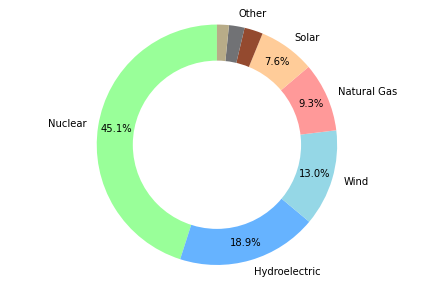
\includegraphics[width=1.0\textwidth]{installed_capacity_france_2020}
	\caption[Share of installed power capacity per energy]{Share of installed power capacity per energy in 2020.}
	\labfig{installed_capacity_france_2020}
\end{figure}


\begin{figure}[hb]
	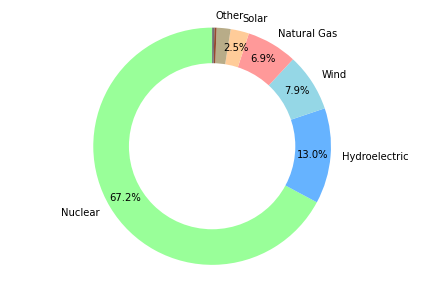
\includegraphics[width=1.0\textwidth]{annual_production_france_2020}
	\caption[Share of 2020 production per energy]{Share of 2020 production per energy.}
	\labfig{annual_production_france_2020}
\end{figure}



We can note that 2020 has been an atypical year in France and the world in general\sidenote[][-2mm]{You don't say!}, with the lowest electricity consumption of the past couple decades. This explains the load factor of nuclear notably being lower than it used to be. This can be seen in the 2019 data shown in~\vreftab{data_2019elec_france}, given here for comparison.

\begin{table*}[ht]
\caption[2019 electricity data for France]{2019 electricity data for France}
\labtab{data_2019elec_france}
\begin{tabular}{ c c c c }
	\toprule
	Type & Installed Capacity (GW) & Energy Produced (TWh) & Load Factor (\%) \\
	\midrule
	Nuclear & 63.1 & 379.5 & 68.7\\
	Coal & 3.0 & 1.6 & 6.1\\
	Petroleum & 3.4 & 2.3 & 7.7\\
	Natural Gas & 12.2 & 38.6 & 36.1\\
	Hydroelectric & 25.6 & 60.0 & 26.8\\
	Solar & 9.4 & 11.6 & 14.1\\
	Wind & 16.5 & 34.1 & 23.6\\
	Biomass & 2.1 & 9.9 & 53.8\\
	\bottomrule
\end{tabular}
\end{table*}


It is important to consider that while some load factors are artificially reduced\sidenote[][*-1]{Nuclear and thermal power plants suffer in part from having to follow the load, and in part due to a market effect}, some are physically limited\sidenote[][*2]{Wind, Solar, and Hydroelectric  generate power only when the wind is blowing, the sun is shining, and sufficient water level is in a reservoir}. France proves to be a good benchmark for a real world case study of nuclear at a large scale, as the lower load factor (in the 60-70\% range, compared to values in the 90\% neighborhood for countries such as the USA, as we will see later) demonstrates the ability of nuclear energy to “load-follow”. On the other hand, production of electricity from solar and wind installed capacity is cheap and even close to free\sidenote[][*1]{Solar and wind indeed do not have any fuel cost, though they do have some maintenance costs}, so a lower value here would be dictated almost entirely by physical limitations in the current market-driven grid.


\begin{kaobox}[frametitle=Load Follow]
Load-Following is the act of quickly adapting the production to the demand by ramping up or down the output of the power plant.
\end{kaobox}

The global demand in France was 473 TWh in 2019 and dropped to 449 TWh in 2020\sidenote[][-2mm]{Impact of lockdowns and a slower economy. Interestingly, one can note that this is lower than the electricity produced in 2019 (537.5 TWh) and in 2020 (500TWh). France is a net exporter of electricity}.


In the near future (horizon 2050), it is likely that due to the electrification of the transportation sector and of the heating sector, the electrical demand in France would rise, though the energy demand would decrease. It is difficult to predict the average use of electricity of a French person then, but we can imagine that better efficiency would imply a lower consumption.

We will assume two main scenarios:

\begin{itemize}
	\item Nuclear Scenario
	\item 100\% Renewable Scenario
\end{itemize}

The Nuclear Scenario will consider that we expand the nuclear program in France to cover 100\% of the electrical demand. The 100\% Renewable Scenario phases out both fossil fuels and nuclear energy from the electricity generation mix. In those scenarios, we are not electrifying the car fleet in the country.

Of course, those scenarios are an exaggeration of what the near future may look like, but it will be interesting to compare their respective viability\sidenote[][-2mm]{Note that no scenarios involving fossil fuels for electricity generation are acceptable, as the end goal is to transition to low carbon energy sources}.

In both scenarios, we can assume that, as a first order approximation, the entire energy capacity need will stay constant and be met by the given resources, that is, the entire annual consumption of 473 TWh. We will come back to this number when the time comes.




\section{United States of America}

This gives the information (2020 and future) for the USA

\section{Brazil}

This gives the information (2020 and future) for Brazil

\section{China}

This gives the information (2020 and future) for China

\section{Nigeria}

This gives the information (2020 and future) for Nigeria

